%mainfile: ../../master.tex
\section{Structure}\label{sub:structure}

\Cref{sec:classes} describes which classes are of relevance in the problem domain. \Cref{sec:events} examines the behaviour of the objects in the problem domain. This section combines the knowledge of these sections to reason about the relations between classes. The relations can be useful later in the design of the system, as understanding the relations between objects will ease the processing of the data observed in the problem domain. \Cref{fig:structure} depicts these relations.

\begin{tikzpicture}
  \begin{class}[text width=2cm]{Location}{0,0}
  \end{class}
  \begin{class}[text width=2cm]{State}{10,0}
  \end{class}
  \begin{class}[text width=2cm]{Time}{0,5}
  \end{class}
  \begin{class}[text width=2cm]{Action}{10,5}
  \end{class}
  \begin{class}[text width=2cm]{Pattern}{0,10}
  \end{class}
  \begin{class}[text width=2cm]{Person}{10,10}
  \end{class}

  \aggregation{State}{ }{1}{Time}
  \aggregation{State}{ }{0..*}{Location}
  \association{Person}{ }{0..1}{Action}{0..*}{ }
  \association{Person}{ }{1}{Pattern}{0..*}{ }
  \association{State}{ }{0..1}{Action}{1}{ }
  \association{Person}{ }{1}{Location}{1}{ }
  \association{Time}{ }{1}{Action}{1}{ }
  \association{State}{ }{1}{Pattern}{1}{ }
  \association{Action}{ }{1}{Location}{1}{ }
  \association{Pattern}{ }{1}{Action}{1..*}{ }
\end{tikzpicture}

% \begin{figure}[htbp]
%   \label{fig:structure}
%   \centering
%   \begin{adjustbox}{max width=\textwidth}
%     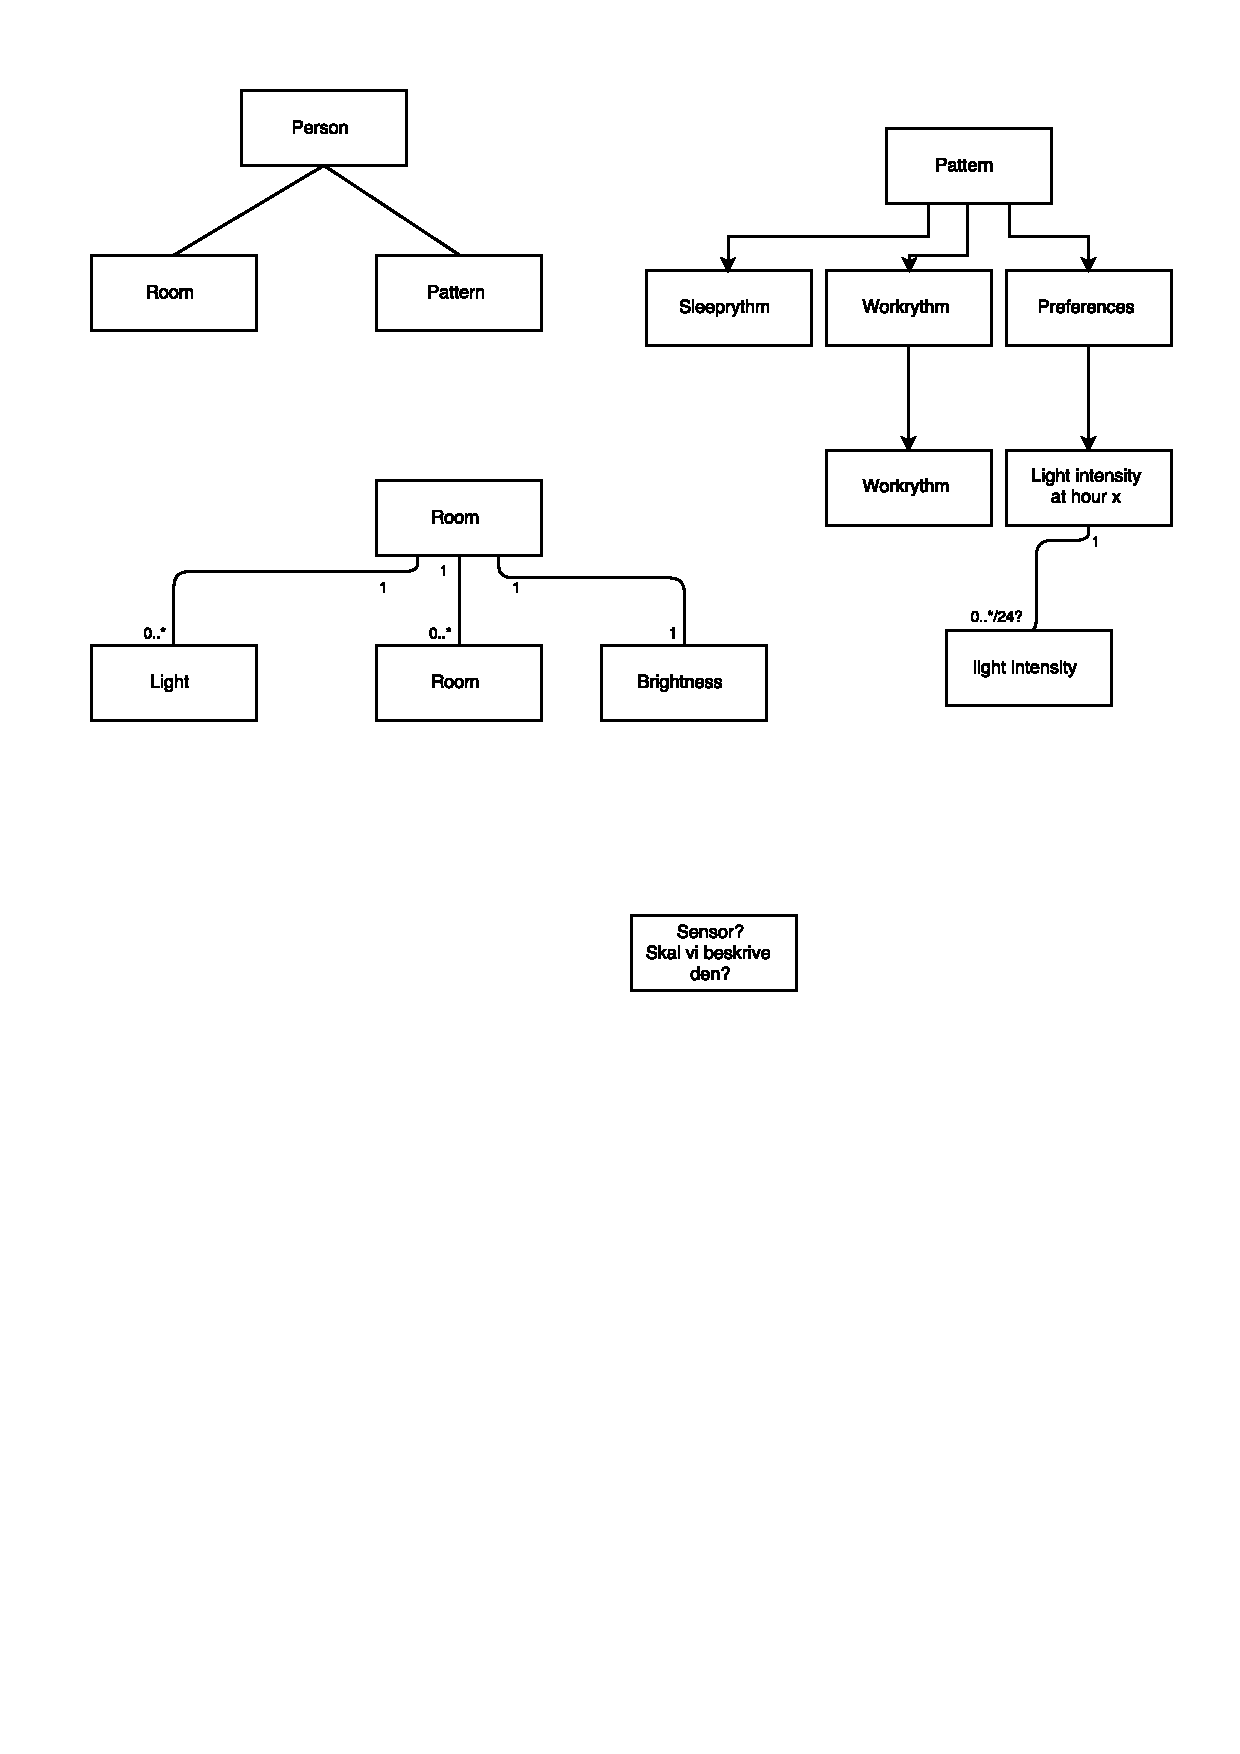
\includegraphics{Structure.pdf}
%   \end{adjustbox}
%   \caption{Structure of the problem domain}\label{fig:structure}
% \end{figure}
